\documentclass[tikz,border=4pt]{standalone}
% Shared style for MultiMM figures (white background, logo palette)
\usepackage{tikz,pgfplots,amsmath}
\pgfplotsset{compat=1.16}
\usetikzlibrary{arrows.meta,calc,decorations.pathreplacing,positioning,backgrounds}
\definecolor{indigo}{HTML}{3B37A0}
\definecolor{violet}{HTML}{6A3AA8}
\definecolor{crimson}{HTML}{B5406C}
\definecolor{gold}{HTML}{E9A62C}
\definecolor{golddark}{HTML}{B9791A}
\definecolor{grey}{HTML}{8A8AA0}
\definecolor{lightgrey}{HTML}{E4E4EE}
\tikzset{
  bead/.style={circle,draw=#1!80!black,fill=#1!35,line width=0.5pt,minimum size=9pt,inner sep=0pt},
  bead/.default=indigo,
  lab/.style={font=\small},
}
\pgfplotsset{
  every axis/.append style={
    width=9.5cm,height=6.3cm,axis lines=left,line width=0.5pt,
    grid=major,grid style={draw=lightgrey,line width=0.3pt},
    tick label style={font=\small},label style={font=\normalsize},
    legend style={font=\footnotesize,draw=none,fill=white,fill opacity=0.8,text opacity=1},
    legend cell align=left,
  },
  every axis plot/.append style={line width=1.2pt,smooth},
}

\begin{document}
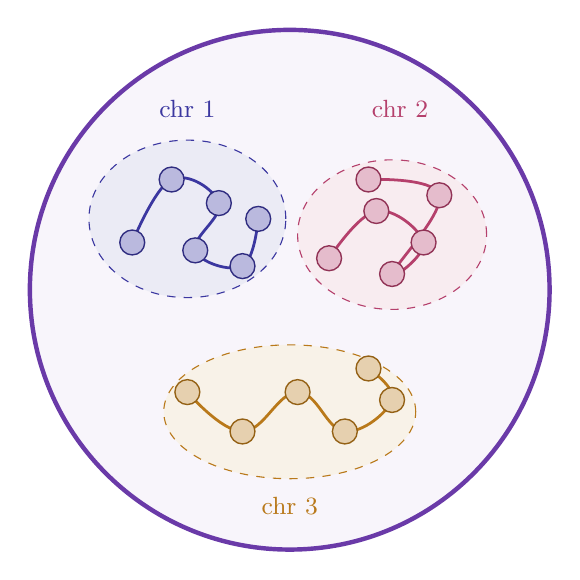
\begin{tikzpicture}
\draw[violet,line width=1.6pt,fill=violet!5] (0,0) circle (3.3);
% three chromosomes, each its own chain and territory
\fill[indigo!10,draw=indigo,dashed] (-1.3,0.9) ellipse (1.25 and 1.0);
\fill[crimson!10,draw=crimson,dashed] (1.3,0.7) ellipse (1.2 and 0.95);
\fill[golddark!10,draw=golddark,dashed] (0.0,-1.55) ellipse (1.6 and 0.85);
\draw[indigo,line width=1pt] plot[smooth,tension=0.7] coordinates {(-2.0,0.6) (-1.5,1.4) (-0.9,1.1) (-1.2,0.5) (-0.6,0.3) (-0.4,0.9)};
\foreach \x/\y in {-2.0/0.6,-1.5/1.4,-0.9/1.1,-1.2/0.5,-0.6/0.3,-0.4/0.9}{\node[bead=indigo] at (\x,\y) {};}
\draw[crimson,line width=1pt] plot[smooth,tension=0.7] coordinates {(0.5,0.4) (1.1,1.0) (1.7,0.6) (1.3,0.2) (1.9,1.2) (1.0,1.4)};
\foreach \x/\y in {0.5/0.4,1.1/1.0,1.7/0.6,1.3/0.2,1.9/1.2,1.0/1.4}{\node[bead=crimson] at (\x,\y) {};}
\draw[golddark,line width=1pt] plot[smooth,tension=0.7] coordinates {(-1.3,-1.3) (-0.6,-1.8) (0.1,-1.3) (0.7,-1.8) (1.3,-1.4) (1.0,-1.0)};
\foreach \x/\y in {-1.3/-1.3,-0.6/-1.8,0.1/-1.3,0.7/-1.8,1.3/-1.4,1.0/-1.0}{\node[bead=golddark] at (\x,\y) {};}
\node[lab,indigo] at (-1.3,2.3) {chr 1}; \node[lab,crimson] at (1.4,2.3) {chr 2}; \node[lab,golddark] at (0,-2.75) {chr 3};
\end{tikzpicture}
\end{document}
